% Official PHreport LaTeX Template
% Written by Karl Welzel
% Last updated on 21 January 2024
% modified by PH
% This document is published under a CC0 1.0 Universal License
% To view a copy of this license, visit http://creativecommons.org/publicdomain/zero/1.0

\documentclass[area=computerscience, review]{PHreportarticle}

\usepackage{amsmath}
\usepackage{amssymb}
\usepackage{pifont}
\usepackage{graphicx}
\usepackage{tabularx}
\usepackage{algorithm}
\usepackage[braket, qm]{qcircuit}
\usepackage{adjustbox}

\newcolumntype{P}[1]{>{\centering\arraybackslash}p{#1}}
\newcolumntype{M}[1]{>{\centering\arraybackslash}m{#1}}

\newcommand{\cmark}{\ding{51}}%
\newcommand{\xmark}{\ding{55}}%

\PHreportinfo{
    title={Inférence Quantique dans les Modèles Graphiques},
    shorttitle={Inférence Quantique},
    author={Thierry Rioual and Tibor Dubois and Mehmet Gunes},
    shortauthor={T. Rioual and T. Dubois and M. S. Gunes},
    authorline={Rioual Thierry \textsuperscript{1}, Dubois Tibor\textsuperscript{2}, Gunes Mehmet\textsuperscript{3}},
    affiliation={
        \item LIP6, Paris (\email{author@upmc.fr})
        \item Math Info (\email{author@gmail.com})
    },
    actor={Pierre-Henri WUILLEMIN},
    function={Encadré par},
    typeofdocument={Rapport de projet},
    publisheddate={2024/03/276},
}

\PHreportheaders{}

\setcounter{page}{1}

\addbibresource{quanticBiblio.bib}

\begin{document}

\maketitle

\begin{PHreportabstractandkeywords}%
    \begin{PHreportkeywords}%
        One,
        Two,
        Three,
        Four,
        Five,
        Six,
        Seven.
    \end{PHreportkeywords}
\end{PHreportabstractandkeywords}

\section*{Avant-propos}

L’émergence de l’informatique quantique, développée à la fin du siècle dernier, nous mène à de nombreuses avancées algorithmiques et computationnelles. A la différence d’un ordinateur classique, un ordinateur quantique fait recours aux principes indéterministes de la mécanique quantique permettant à la machine de réaliser plusieurs opérations en parallèle. 
Cela donne lieu à la création d'algorithmes quantiques qui nous permet d’aborder des problèmes non-envisageables auparavant avec les algorithmiques classiques. 
L’inférence dans les modèles graphiques, les réseaux bayésiens en particulier, est connue pour être un problème NP-difficile, nécessitant des algorithmes sophistiqués. Ce projet vise à explorer l’application de la programmation quantique à ce domaine spécifique.
\\
Dans un premier temps, nous réaliserons une présentation succincte des réseaux bayésiens. Ensuite, sans préoccupation de la physique quantique à l’issue des machines quantiques, nous introduirons les rudiments de l’informatique quantique. 
\section{État de l'art}

\subsection{Introduction aux réseaux bayésien}
\label{IntroBN}

Un réseau bayésien est une distribution jointe de probabilité sur une famille \( (X_1,...,X_n) \) de variables aléatoires discrètes. Cette distribution est décrite par un \textit{graphe orienté sans circuit} ou DAG (Directed Acyclic Graph), et un ensemble de \textit{tables de probabilités conditionnelles} ou CPT (Conditional Probability Table). Les sommets du graphe représentent les variables aléatoires en question, et les arcs sont les dépendances conditionnelles entre les différentes variables.
\\
Dans un graphe orienté, on distingue trois types de relations entre un nœud \(\mathrm{X}\) et ses voisins, on dit que: 
\begin{itemize}
\centering
    \item \(\mathrm{Y}\) est un parent de \(\mathrm{X}\) si:  \quad\(\mathrm{Y} \rightarrow \mathrm{X} \)
    \item \(\mathrm{Z}\) est un enfant de \(\mathrm{X}\) si:  \quad\(\mathrm{Z} \leftarrow \mathrm{X} \)
    \item \(\mathrm{S}\) est une épouse de \(\mathrm{X}\) si:  \quad\(\mathrm{S} \rightarrow \mathrm{Z} \leftarrow \mathrm{X} \)
\end{itemize}

\noindent Où \(\mathrm{A} \rightarrow \mathrm{B} \) représente une arrête du noeud \(\mathrm{A}\) vers le noeud \(\mathrm{B}\). Dans ce dernier cas, \(\mathrm{S}\) est aussi un parent de \(\mathrm{Z}\). Les épouses sont définies comme des nœuds qui partagent au moins un enfant en commun et ne partageant entre eux aucun autre lien direct. (\cite{FouillesMassivesSoins})
\\
Ainsi, dans le cadre d'un réseau bayésien, si \(X_j\) est un parent de \(X_i\), alors \(X_i\) est dépendant de \(X_j\). En définissant \( Pa(X_i) \subseteq \{X_1,..., X_n\} \) comme l'ensemble des parent de \(X_i\), on retrouve \(P(X_i | Pa(X_i))\), la loi de \(X_i\) conditionnellement à l’état de ses parents \(Pa(X_i)\). C'est précisément cette loi que décrit le CPT associé au sommet de \(X_i\). Toutes les variables sont donc conditionnellement indépendante de leur non-descendant, sachant ses parents, on dit en autres qu'elles vérifient la \textit{propriété de Markov}. (\cite{gene_network})
\\
On retrouve ainsi la probabilité jointe de la famille \((X_1,..., X_n)\) de variables aléatoires par la formule des probabilités composées:
\begin{equation}
\label{eq:1}
    P(X_1,..., X_n) = \prod_{i=1}^{n}P(X_i | Pa(X_i))
\end{equation}
Un avantage capital des réseaux bayésiens se trouve dans leur capacité à représenter de manière succincte des distributions multidimensionnelles, sans tomber dans l'explosion combinatoire. En effet, en passant par une étude de graphes, le nombre de paramètre à calculer est réduit conséquemment grâce à la factorisation (\ref{eq:1}).
\begin{figure}
\centering
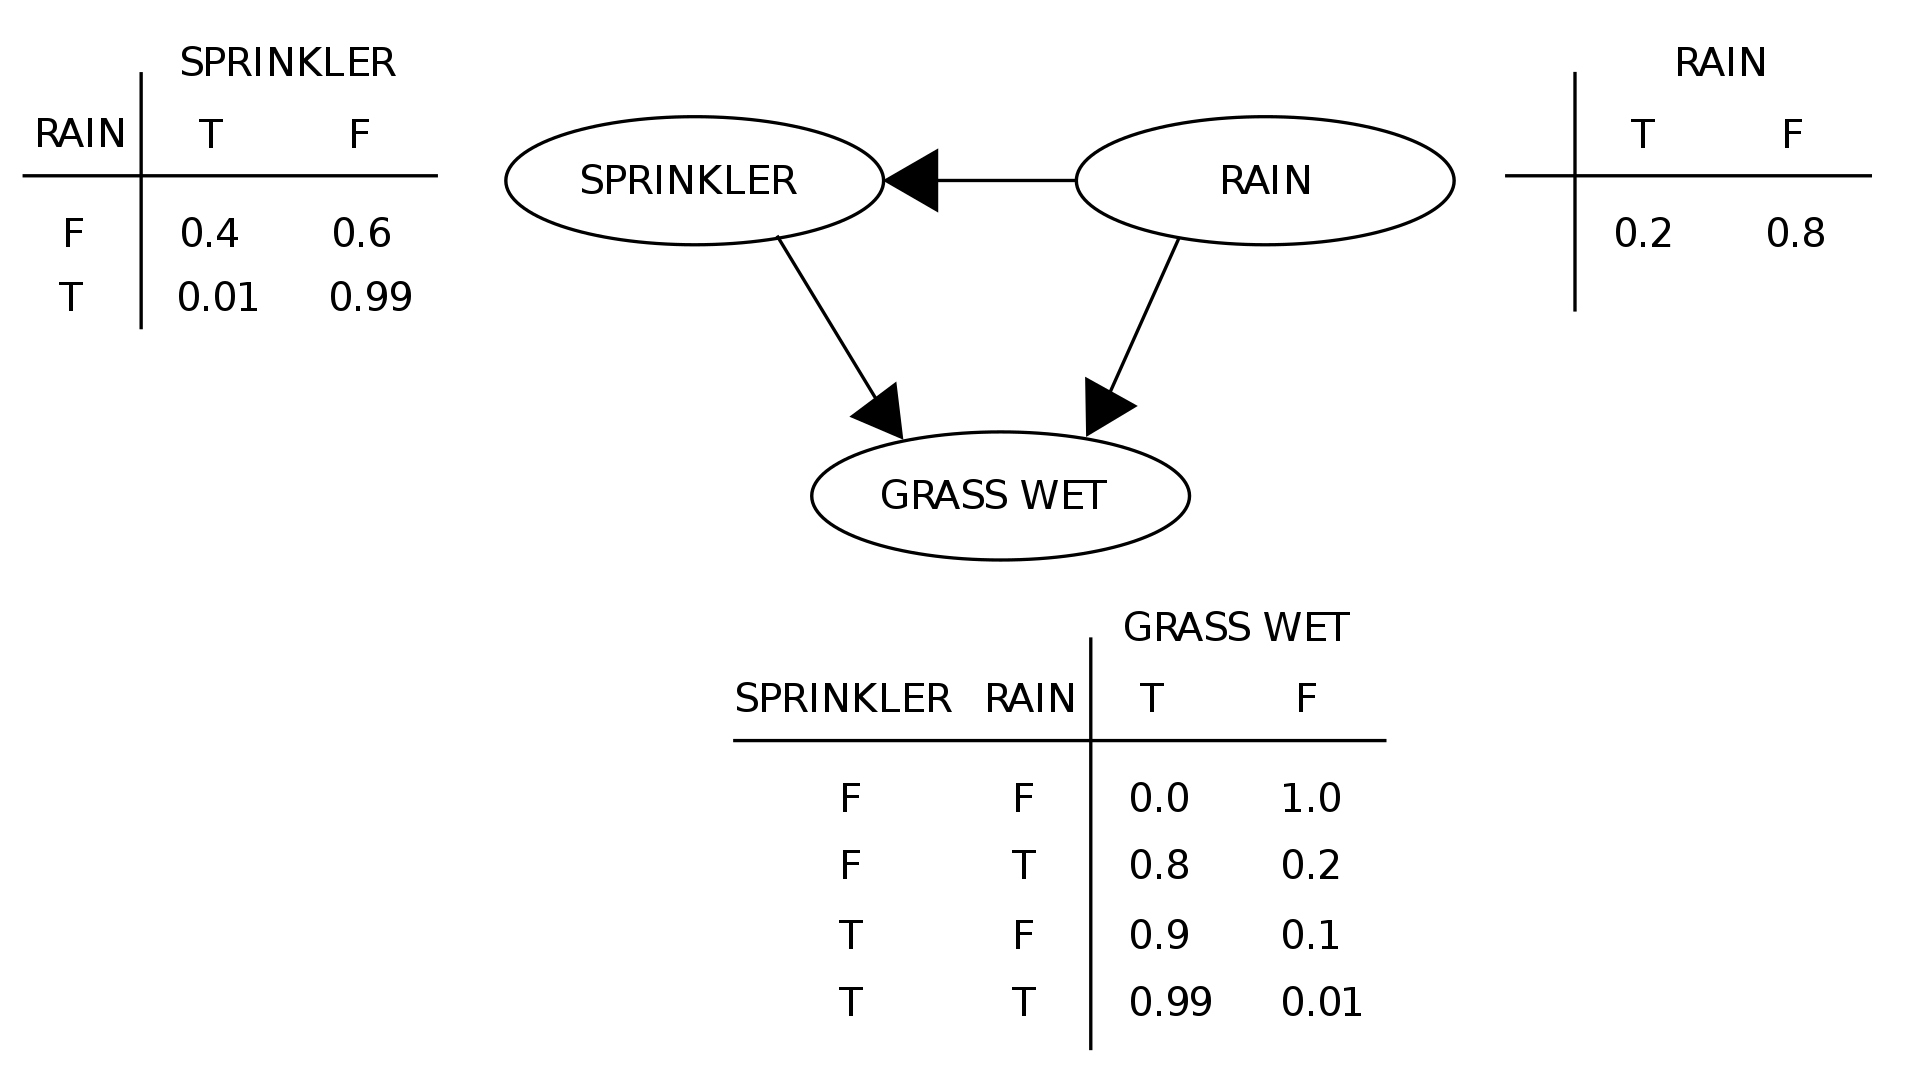
\includegraphics[scale=0.18]{SimpleBayesNet.png}
\caption{Exemple d'un réseau bayésien avec trois arrêtes}
\label{fig:ExBN}
\end{figure}
%Dans l'exemple de la figure \ref{fig:ExBN}, 

\subsection{Introduction à l'informatique quantique}
\label{IntroQuant}

Similairement au bit de la théorie de l’information classique, l’information quantique se base sur la manipulation de bits quantiques, appelés \textit{qubits}. Cependant, l’espace d’état de ces derniers diffère de leur homologue classique dû au fait que nous retrouvons, en plus des états \(0\) et \(1\), les états de superposition, dans lesquelles les qubits en question peuvent être dans les deux états simultanément avant d’être mesurés (ou observés). En pratique, les qubits sont représentés par les vecteurs unitaires de \(\mathbb{C}^2 \) muni du produit scalaire hermitien. L’état \(|0\rangle\), représenté par le vecteur \((1\;0)\) et l’état \(|1\rangle\) par \((0\;1)\), sont les bits classiques et forment la base canonique de l’espace vectoriel. 
\\
Tout qubit \(|\psi\rangle\) s’exprime donc par une combinaison linéaire : 
\begin{equation}
|\psi\rangle = \alpha|0\rangle +\beta|1\rangle \quad \text{tel que} \quad (\alpha,\beta) \in \mathbb{C}^2 , \; |\alpha|^2 + |\beta|^2 = 1
\end{equation}

\noindent La mesure d’un qubit entraîne le phénomène de réduction, qui réduit un qubit superposée en un bit classique, elle entraîne en outre la destruction de l’information quantique contenu dans le qubit. Le module au carré de chacune des deux coordonnées du qubit dans \(\mathbb{C}^2 \) représente ainsi les probabilités respectives de \(0\) et \(1\) lors de la mesure, ce qui illustre le principe de superposition. D’un point du vue probabiliste, le fait que le vecteur du qubit soit unitaire nous assure que les probabilités associées aux états classiques forment un système complet d'événements. Géométriquement, la visualisation d’un qubit se fait à travers la sphère de Bloch, celle-ci permet d’étudier les qubits du plan \(\mathbb{C}^2 \) sous la structure algébrique de \(\mathbb{R}^3 \) en utilisant les coordonnées sphériques. 
\\
\begin{figure}
\centering
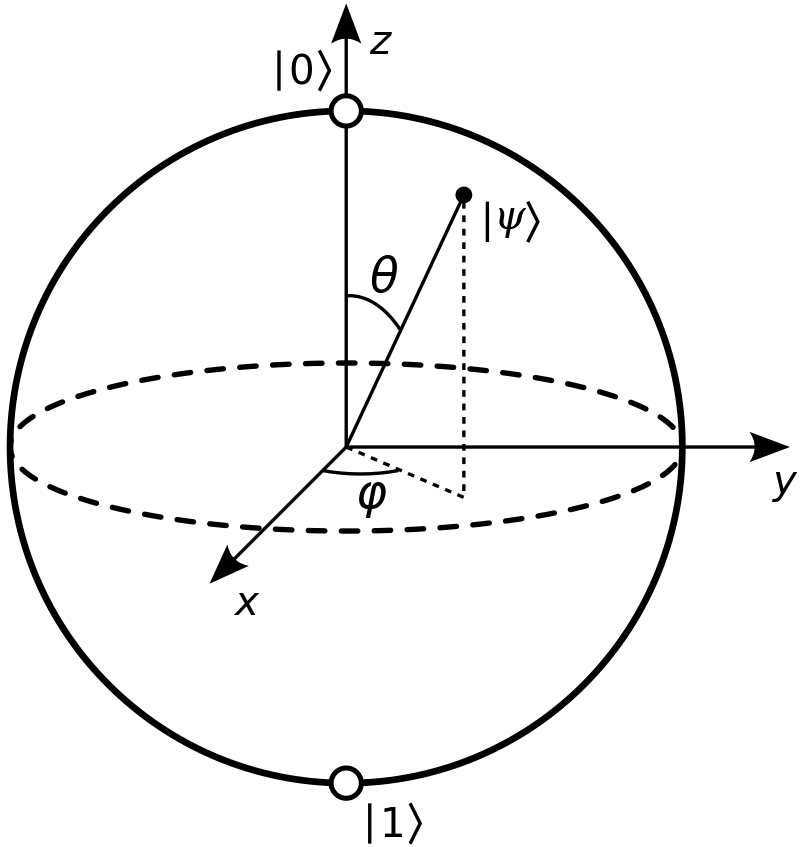
\includegraphics[scale=0.15]{Bloch_sphere.png}
\caption{La Sphère de Bloch}
\label{fig:Bloch}
\end{figure}
\noindent Nous développerons ici des algorithmes quantiques sous le modèle de circuits quantiques, qui réalisent les opérations sur les qubits séquentiellement. Ces opérations sont effectuées par les portes quantiques représentées par les opérateurs unitaires de \(\mathbb{C}^2 \) sous la forme de \(U(\theta, \phi, \lambda)\), qui sont analogues aux portes logiques pour les circuits électroniques classiques. On retrouve notamment la porte NOT ou \(X\), mais aussi \(R_Y\) et \(R_Z\) qui représentent une rotation selon l’axe X, Y et Z respectivement dans la sphère de Bloch, celles-ci sont aussi appelées \textit{portes de rotations}. (\cite{quant_rep_BN})
\begin{equation}
\mathrm{U}(\theta, \phi, \lambda) = 
\begin{bmatrix}
cos(\frac{\theta}{2}) & -e^{i\lambda}sin(\frac{\theta}{2}) \\
e^{i\phi}sin(\frac{\theta}{2}) & e^{i(\phi + \lambda)}cos(\frac{\theta}{2})
\end{bmatrix}
, \quad 
(\theta, \phi, \lambda) \in [0,\pi] \times [0, 2\pi]^2
\end{equation}
Pour réaliser des opérations concernant de multiples qubits, nous faisons recours au \textit{produit tensoriel}, qui est un moyen commode de coder les objets multilinéaires. En pratique, les portes $X$ et $R_Y$ contrôlée ($CNOT$ et $CR_Y$) seront utilisées principalement. Celles-ci agissent sur un qubit de contrôle et un qubit cible ; quand le qubit de contrôle vaut \(0\), le qubit cible reste inchangée, tandis que lorsqu’il vaut \(1\), la porte \(X\) (ou $R_Y$) est appliquée sur le qubit cible. Il est possible d’exprimer la version contrôlée d’une opération unitaire \(U\) quelconque comme une combinaison de porte \(CX\) et de porte agissant sur un seul qubit. Plus généralement, ces opérations engendrent les portes 
\(C^nU\)  ayant n qubits de contrôle et un qubit cible. Celles-ci appliquent l’opération \(U\) sur le qubit cible lorsque tous les n-qubits valent \(1\), et constituent toutes les opérations que nous utiliserons dans ce projet.

\begin{equation}
CX = 
\begin{bmatrix}
1&0&0&0\\
0&1&0&0\\
0&0&0&1\\
0&0&1&0\\
\end{bmatrix}
, \quad 
CU = 
\begin{bmatrix}
1&0&0&0\\
0&1&0&0\\
0&0&cos(\frac{\theta}{2}) & -e^{i\lambda}sin(\frac{\theta}{2}) \\
0&0&e^{i\phi}sin(\frac{\theta}{2}) & e^{i(\phi + \lambda)}cos(\frac{\theta}{2})
\end{bmatrix}
\end{equation}


\subsection{Approche à un problème NP-difficile}
\label{QuantRepBN}


Le cadre du projet se porte sur l'inférence dans les réseaux bayésien, c'est-à-dire la détermination de la probabilité postérieure d'un ensemble de variables étant donné certaines observations. L'inférence exacte requiert dans les pires des cas une sommation sur un nombre exponentiel de configurations de variables, il s'agit d'un problème \textit{NP-difficile}.\footnotemark
\\
L'exploration exhaustive des configurations structurelles possibles contraintes par un critère d'optimisation tel que la vraisemblance, devient rapidement une tâche herculéenne. À mesure que le nombre de variables s'accroît, il y a une augmentation exponentielle du nombre de structures à évaluer, rendant ainsi le processus de sélection impraticable. Afin de tirer avantage des temps de calcul réduits des ordinateurs quantiques, nous allons construire des circuits quantiques qui représenteront des réseaux bayésien afin d'évaluer leur performances inférentielles.
\\
Plus concrètement, nous aborderons le problème d'inférence à travers 
l'échantillonnage par rejet avec la méthode de Monte-Carlo. Pour un réseau 
bayésien à $k$ variables ayant chacune moins de $m$ parents, la génération d’échantillons classiques de la loi jointe se fait en $\mathcal{O}(km)$. Ainsi pour $P_e$ la probabilité de l’observation, la méthode de rejet possède une complexité en espérance de $\mathcal{O}(km/P_e)$. La performance computationnelle de l’algorithme classique se dégrade des lorsque $P_e$ devient faible, c'est-à dire lorsque le nombre de variables observées augmente.
\\
Notre objectif est donc de reformuler la problématique d'échantillonnage en un problème pour lequel l'algorithmique quantique présente un avantage considérable : la recherche non structurée, pour obtenir une complexité finale de $\mathcal{O}(k2^m/\sqrt{P_e})$. 


\footnotetext{Dans la théorie de la complexité informatique, la classe de problème non déterministe polynomial NP contient les problèmes dont on peut vérifier si une solution est candidate en temps polynomial. On dit alors qu'un problème H est NP-difficile, si tout problème L de la classe NP peut être réduit en temps polynomial à H. C'est-a-dire on peut transformer en temps polynomial, la résolution de H en résolutions de problèmes NP.}
\section{Cahier des charges}

\subsection{Environnement de programmation quantique}
\label{MedProg}
La programmation quantique, fondée sur l'informatique quantique, est le processus de conception et d’assemblage de circuits quantiques (c.f. \ref{IntroQuant}), qui, en manipulant un système de qubits, aboutiront à un certain résultat. Il existe de nombreux moyens de procéder à la programmation quantique, dans cette section, nous comparerons ces différents moyens afin d’aboutir à un environnement de programmation sur lequel se basera le reste du projet.
\\
Les environnements de programmation quantique peuvent être regroupées en trois principales catégories:

\begin{itemize}
\item Les \textit{jeux d'instructions quantiques} (Quantum Instruction Sets) permettent de traduire un algorithme de haut niveau en instructions physique qui pourront être exécutées sur des processeurs quantiques.
\item Les \textit{langages de programmation quantique} sont des langages dédiés à écrire des programmes pour un ordinateur quantique.
\item Les\textit{ kits de développement de logiciels quantiques} ou SDK (Quantum Software Development Kit) contiennent une collection d’outils de création et manipulation de programme quantiques dans un package installable.
\end{itemize}

\noindent Afin de nous concentrer sur le cœur du sujet, nous avons décidé de dévouer notre attention sur les SDK qui permettront une approche de haut niveau à la programmation quantique. En effet, la plupart de ces packages se basent sur le langage Python, omniprésent dans la communauté scientifique depuis les 30 dernières années. Plus récemment, de multiples géants de la technologie investissent dans l’informatique quantique et proposent leur propre SDK, nous travaillerons ici avec Qiskit, proposé par IBM. 
\\

\begin{table}
\begin{tabular}{|M{3cm}||M{2.5cm}|M{2.5cm}|M{2.5cm}|M{2.5cm}|}
    \hline
    Critère & Qiskit (IBM) & Cirq (Google) & ProjectQ (ETHZ) & Forest (Rigetti) 
    \\ \hline
    Compilation sur ordinateur Quantique & 
    \cmark & \xmark & \xmark & \xmark \\ \hline
    Communauté & 
    6.55M Downloads, Chaines Youtube, 543 Contributors, GitHub repo & 
    Stack Exchange, QuantumLib repo & 
    Github Repo, Documentation, Online Forums &
    Github Repo, Documentation, Online Forums
    \\ \hline
    Bilbiothèques & 
    Qiskit Terra, Aer, Ignis, Aqua, Finance & TensorFlow Quantum & \xmark & \xmark
    \\ \hline
    GUI & 
    IBM Quantum Experience & Quirk & \xmark & \xmark 
    \\ \hline
\end{tabular}
\caption{Comparaison entre les languages}\label{comp}
\end{table}

\noindent 
Qiskit semble être un excellent choix pour la programmation quantique pour plusieurs raisons. Tout d'abord, il bénéficie du soutien robuste d'IBM, l'un des leaders de l'informatique quantique. Avec plus de 6,55 millions de téléchargements, une communauté dynamique, et une présence active sur des plateformes comme YouTube, il offre un écosystème riche pour l'apprentissage et l'échange entre utilisateurs. 
De plus, Qiskit possède une riche bibliothèque qui comprend Terra pour la construction de circuits quantiques, Aer pour la simulation, Ignis pour l'atténuation des erreurs, Aqua pour les applications quantiques, et une multitude d’autres concernant le domaine de la finance par exemple. Cette gamme complète de fonctionnalités fait de Qiskit un outil versatile dans le domaine quantique. En comparaison, Google associe a son language une bibliothèque de machine learning quantique, Tensor Flow Quantum. Celle-ci permet le prototypage rapide de modèles d'apprentissage machine hybrides, cependant, cela ne rentre pas dans le cadre de notre recherche.
\\
La représentation graphique des circuits quantiques dans Qiskit est également un point fort, permettant aux utilisateurs de visualiser et de déboguer les circuits de manière intuitive. L'IBM Quantum Experience offre une plateforme accessible pour l'exécution de circuits sur des simulateurs et des ordinateurs quantiques réels. 
Enfin, l'aspect open-source de Qiskit, avec son importante équipe de contributeurs de GitHub, assure une évolution constante et une amélioration continue du framework, le rendant à la pointe de la technologie quantique.

\subsection{Introduction à pyAgrum}

Tout d’abord, aGrUm est une librairie C++ créée en 2008 pour les modèles graphiques probabilistes, portant principalement sur la représentation des réseaux bayésiens, mais aussi d’autres modèles tels que les réseaux crédeaux, les modèles probabilistes relationnels, diagrammes d’influences ou encore les chaînes de Markov. C’est un choix intéressant pour sa performance apportée par le C++ et sa précision, le menant à être utilisé par des laboratoires de recherches comme LIP6, des startups et des géants industriels tels que EDF, Airbus et IBM.
\\
Ultérieurement, pyAgrum est un wrapper Python pour la libraire aGrUm, rendant cette librairie qui est de source C++ plus accessible grâce à l’intermédiaire de Python. Fournissant un environnement d’analyse et de modélisation probabiliste à l’utilisateur qui peut implémenter à travers des Notebook comme Jupyter Notebook. L’avantage de pyAgrum est qu’il combine la présence d'une interface graphique avec la maniabilité du code telle qu’on la connaît.

\subsection{Cas d'usage}

Plutôt que de fournir un cahier des charges détaillé, nous décrivons les cas d'usage de la librairie que nous devons créer durant ce projet.

Avec pour objectif de mettre en œuvre l'inférence de Réseaux Bayésiens en utilisant des méthodes classiques et quantiques, nous avons conçu diverses classes pour gérer différents aspects des RB, notamment leur construction, leur modification et leur processus d'inférence.

\subsection*{1. \texttt{qBNMC}}
\begin{itemize}
    \item \textbf{Initialisation} : 
    \begin{minipage}{\linewidth}
    \begin{lstlisting}
    qbn = qBNMC(bn)
    \end{lstlisting}
    \end{minipage}
    
    % Ici, bn est un Réseau Bayésien créé et chargé en utilisant une bibliothèque telle que pyAgrum. Cette étape permet de transformer le modèle probabiliste classique en un modèle compatible avec l'inférence quantique.
    
    \item \textbf{Méthodes} :
    \begin{itemize}
        \item \texttt{getProbability} : Calcule la probabilité qu’un qubit prenne une valeur donnée, en tenant compte des autres qubits représentant la variable et d’autres nœuds du Réseau Bayésien.
        \item \texttt{multiQubitRotation} : Ajoute au circuit quantique une série de rotations qui mappent les probabilités de la variable aux qubits correspondants, en fonction des états des qubits contrôleurs.
        \item \texttt{buildCircuit} : Construit le circuit quantique à partir du Réseau Bayésien, en incluant les rotations et les connexions nécessaires entre les qubits.
        \item \texttt{aerSimulation} : Exécute une simulation du circuit quantique du Réseau Bayésien en utilisant le simulateur Aer, et retourne les résultats de la mesure des qubits.
        \item \texttt{runBN} : Construit et exécute le circuit quantique représentant le Réseau Bayésien, et retourne les potentiels associés à chaque variable du réseau.
    \end{itemize}
\end{itemize}

\subsection*{2. \texttt{qBNRejection}}
\begin{itemize}
    \item \textbf{Initialisation} : 
    \begin{minipage}{\linewidth}
    \begin{lstlisting}
    qinf = qBNRejection(qbn)
    \end{lstlisting}
    \end{minipage}
    
    % L'initialisation de cette classe nécessite une instance de qBayesNet représentant le Réseau Bayésien quantique.

    \item \textbf{Méthodes} :
    \begin{itemize}
        \item \texttt{getGates} : Prépare les portes A et G pour l'échantillonnage par rejet.
        \item \texttt{transpileGates} : Transpile les portes A et G pour optimiser le circuit quantique.
        \item \texttt{getEvidenceQuBits} : Donne la représentation en qubits de l'évidence dans le Réseau Bayésien.
        \item \texttt{getSample} : Génère un échantillon basé sur les évidences données.
        \item \texttt{makeInference} : Exécute l'échantillonnage par rejet sur le circuit quantique représentant le Réseau Bayésien.
        \item \texttt{setEvidence} : Définit les évidences pour l'inférence, en ajustant les états initiaux du circuit quantique en conséquence.
        \item \texttt{posterior} : Donne la table de probabilité d'une variable basée sur les résultats de l'échantillonnage.
        \item \texttt{useFragmentBN} : Utilise un fragment du Réseau Bayésien pour l'inférence, en se concentrant uniquement sur les variables ciblées. 

    \end{itemize}
\end{itemize}

\subsection*{3. \texttt{qRuntime}}
\begin{itemize}
    \item \textbf{Initialisation} : 
    \begin{minipage}{\linewidth}
    \begin{lstlisting}
    qrt = qRuntime(backend, qinf)
    \end{lstlisting}
    \end{minipage}
    
    % L'initialisation de cette classe nécessite un backend quantique (comme ceux fournis par IBM Quantum) et une instance de qInference. Cela permet de préparer le cadre pour l'évaluation comparative des performances.

    \item \textbf{Méthodes} :
    \begin{itemize}
        \item \texttt{getAtime} : Estime le temps d'exécution théorique du circuit quantique pour une porte donnée sur un backend quantique.
        \item \texttt{getGtime} : Estime le temps d'exécution théorique d'une itération de Grover sur un backend quantique.
        \item \texttt{rejectionSamplingRuntime} : Utilise le temps d'exécution des portes pour calculer le temps total du processus d'échantillonnage par rejet.
    \end{itemize}
\end{itemize}



\section*{Exemple de Flux de Travail}

\subsection*{Étape 1 : Charger et Afficher le Réseau Bayésien}
Charger un Réseau Bayésien en utilisant \texttt{pyAgrum} et le visualiser.
\begin{verbatim}
import pyAgrum as gum
import pyAgrum.lib.notebook as gnb

bn = gum.loadBN("path_to_your_bayesian_network.bif") 
gnb.showBN(bn, size=20)
\end{verbatim}

% Ici, bn est le Réseau Bayésien chargé depuis un fichier. Remplacez "path_to_your_bayesian_network.bif" par le chemin de votre fichier RB.

\subsection*{Étape 2 : Construire un Réseau Bayésien Quantique}
Créer une instance de \texttt{qBayesNet} avec le Réseau Bayésien chargé.
\begin{verbatim}
qbn = qBayesNet(bn)
\end{verbatim}

% Cette étape crée un modèle quantique à partir du Réseau Bayésien classique.

\subsection*{Étape 3 : Modifier et Générer une CPT}
Générer une Table de Probabilités Conditionnelles (CPT) aléatoire pour les nœuds du Réseau Bayésien.
\begin{verbatim}
def getRandomBinaryCPT(num_parents):
    # Code pour générer une CPT aléatoire
    pass

# Exemple d'utilisation
for n_id in bn.nodes():
    bn.cpt(n_id)[:] = getRandomBinaryCPT(len(bn.parents(n_id)))
\end{verbatim}

% Cette fonction génère des CPTs aléatoires pour les nœuds du RB, où num_parents représente le nombre de parents d'un nœud.

\subsection*{Étape 4 : Effectuer l'Inférence Quantique}
Initialiser la classe \texttt{qInference} et exécuter l'inférence.
\begin{verbatim}
qinf = qInference(qbn)
qinf.runInference(backend)
\end{verbatim}

% backend représente le backend quantique utilisé pour l'inférence (par exemple, un backend d'IBM Quantum).

\subsection*{Étape 5 : Évaluer le Temps d'Exécution}
Utiliser \texttt{qRuntime} pour évaluer et comparer les temps d'exécution.
\begin{verbatim}
qrt = qRuntime(backend, qinf)
qrt.run()
\end{verbatim}

% qRuntime permet de mesurer et comparer les temps d'exécution des inférences classiques et quantiques.

\subsection*{Étape 6 : Visualiser les Résultats}
Générer des graphiques pour comparer la performance des inférences Monte Carlo (MC) et Quantique (QI).
\begin{verbatim}
import matplotlib.pyplot as plt

# ev_prob_list : Liste des probabilités d'évidence.
# mc_rt_list : Liste des temps d'exécution pour Monte Carlo.
# qinf_rt_list : Liste des temps d'exécution pour l'inférence quantique.

# Exemple de Code pour tracer les graphiques
# Affiche les temps d'exécution pour Monte Carlo
plt.scatter(ev_prob_list, mc_rt_list, color="tab:orange", label="Temps d'exécution MC") 
# Affiche les temps d'exécution pour l'inférence quantique
plt.scatter(ev_prob_list, qinf_rt_list, color="tab:blue", label="Temps d'exécution QI") 
# Utilise une échelle logarithmique pour l'axe Y
plt.yscale('log')  
plt.xlabel('Probabilité d\'évidence')  
plt.ylabel('Temps d\'exécution')  
plt.legend()  
plt.show() 
\end{verbatim}

% ev_prob_list représente la liste des probabilités d'évidence, mc_rt_list les temps d'exécution pour Monte Carlo et qinf_rt_list les temps d'exécution pour l'inférence quantique.






\iffalse
\begin{lstlisting}
import pyAgrum as gum
import pyAgrum.lib.quantik as gqt

# From BN to QC
bn=gum.fastBN('A->B{yes|no}->C',5)

#for v in bn.names():
#  print(bn[v])
#  print(bn[v].domainSize())
#  print(bn.cpt(v))

qbn=qgt.qBN(bn)
print(qbn.qbytes())
circuit=qbn.toqiskit()

qie = qgt.qRejectSampling(bn)
qie.addEvidence("C",3)
qie.setEpsilon(1e-5)
qie.setTimeout(5)
cinference=qie.toqiskit() 
\end{lstlisting}
\fi
\section{Algorithmes et Implémentations}

Dans le cadre des contraintes de brièveté de ce rapport, l'explication détaillée des algorithmes, incluant un formalisme mathématique adéquat, sera présentée en annexe. Ici, nous nous contenterons de présenter les principales idées. %1

\subsection{Amplification d'amplitude}

%L'article de \cite{grover1996fast} est une publication majeure en informatique quantique. L'algorithme de Grover décrit dans ce papier introduit la technique d'\textit{amplification d'amplitude}, qui accélère divers algorithmes classiques. Les algorithmes d'amplification d'amplitude sont des algorithmes de recherche non structurée quantiques permettant de trouver un ou plusieurs éléments appelés \textit{solutions} parmi un ensemble de $N$ éléments avec une complexité de $\mathcal{O}(\sqrt{N})$, comparée à $\mathcal{O}(N)$ pour un algorithme classique, voire même probabiliste. 

L'article de \cite{grover1996fast} constitue une publication majeure en informatique quantique. L'algorithme décrit dans ce papier, désormais connu sous le nom d’algorithme de Grover, introduit la technique d'\textit{amplification d'amplitude}, permettant d'accélérer divers algorithmes classiques. Les algorithmes d'amplification d'amplitude sont des algorithmes de recherche non structurée qui permettent de trouver un ou plusieurs éléments appelés \textit{solutions} parmi un ensemble de $N$ éléments avec une complexité de $\mathcal{O}(\sqrt{N})$, comparée à $\mathcal{O}(N)$ pour un algorithme classique. 
\\
Notons que l'ensemble de recherche n'a aucune structure exploitable, sinon, si l'ensemble était trié par exemple, une recherche dichotomique classique offrirait une complexité de $\mathcal{O}(\mathrm{log}(N))$ meilleure que celle proposé par l'algorithme de Grover. La technique d'amplification d'amplitude repose sur la représentation de l'ensemble de recherche par un système quantique, où chaque qubit correspond à un élément de l'ensemble. Ce système est décrit par un espace vectoriel décomposé en deux sous-espaces: l'un contenant les solutions et l'autre, son orthogonal, les non-solutions. L'algorithme commence par la superposition de tous les vecteurs d'états du système quantique, puis applique des rotations unitaires pour amplifier l'amplitude des états correspondant aux solutions et réduire celles des non-solutions. Ces rotations incluent des opérations de diffusion $U_{\psi}$ et d'inversion $U_{\omega}$, orientant progressivement le vecteur de superposition vers le sous-espace des solutions.
\\
À chaque étape, la probabilité d'observer une solution lors de la mesure finale augmente. L'objectif est d'optimiser cette probabilité pour qu'il soit très probable d'obtenir un état correspondant à une solution du problème de recherche lors de la mesure du système quantique. Une explication détaillé de ce processus est détaillée dans l'annexe. %2

\begin{figure}[H]
\centering
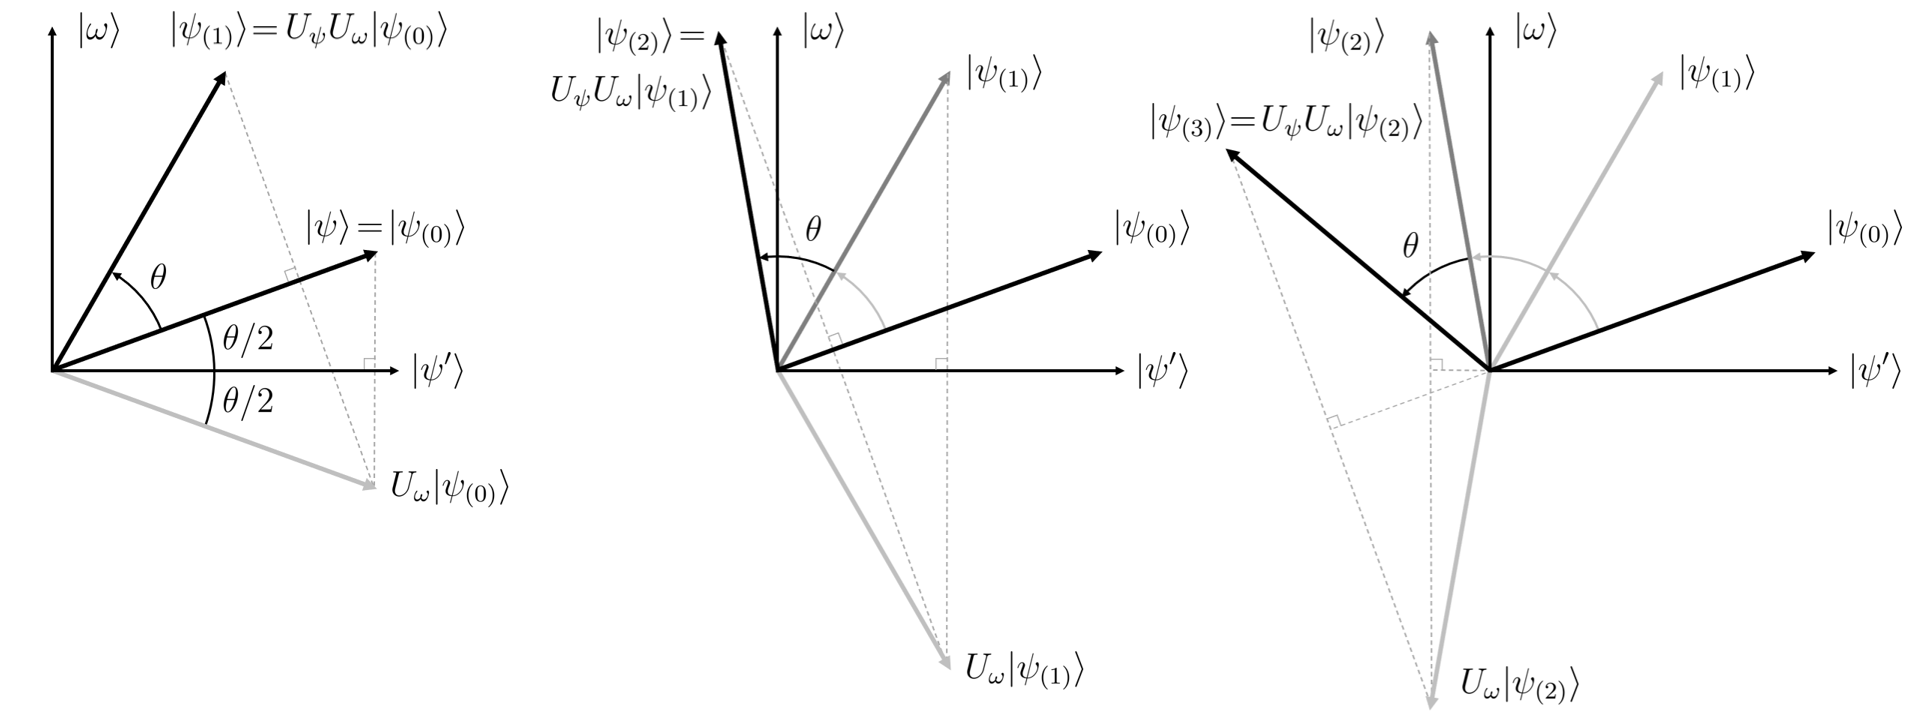
\includegraphics[scale=0.30]{GroverGeom.png}
\caption{Interprétation géométrique de l'algorithme de Grover}
\label{fig:GroverGeom}
\end{figure}
\noindent

\subsection{Préparation d'un q-échantillon}
\label{prepQE}
Pour exploiter les améliorations de complexité des algorithmes quantiques, il est nécessaire de pouvoir représenter un réseau bayésien par un circuit quantique. L'article de \cite{quant_rep_BN} propose une méthode pour générer des \textit{q-échantillons}, des vecteurs d'état représentant les échantillons de la distribution de probabilité du réseau bayésien.
\\
En bref, la préparation des q-échantillons s'effectue en trois principales étapes:
\begin{itemize}
    \item[1] Associer chaque variable du réseau bayésien à un ou plusieurs qubits (en fonction du nombre de valeurs prises par la variable).
    \item[2] Associer les probabilités (marginales ou conditionnelles) de chaque variable aux amplitudes des états composantes des qubits correspondants.
    \item[3] Encoder les amplitudes des états quantiques en utilisant des portes de rotation (contrôlées), dans un ordre topologique du graphe.
\end{itemize}
\noindent
Considérons d'abord un réseau bayésien composé de variables binaires. L'algorithme représente chaque variable par un qubit et effectue des rotations sur ces qubits pour leur attribuer la distribution de la table de probabilité conditionnelle (CPT) de la variable. Pour les racines du graphe, ce processus est directe, car la CPT a seulement deux entrées, correspondant aux états $|0\rangle$ et $|1\rangle$ d'un qubit. Pour les variables ayant des parents, il faut appliquer une série de rotations conditionnées par toutes les combinaisons de valeurs des parents. L'ordre des rotations est crucial, car les probabilités d'une variable dépendent de celles de ses parents; ainsi, les rotations doivent suivre un ordre topologique du graphe. 
\\
Pour les variables aléatoires discrètes pouvant prendre plusieurs valeurs, il faut binariser ces valeurs et utiliser plusieurs qubits pour représenter chaque variable. Les rotations sont plus complexes car elles impliquent plusieurs qubits. Il est donc nécessaire de procéder par étapes, en se concentrant sur un qubit à la fois. L'approche consiste à s'inspirer des rotations appliquées aux variables ayant des parents pour effectuer une binarisation de la variable discrète.
\\
La réalisation concrète de cette étape nécessite l'utilisation d'une fonction indicatrice et d'une fonction de binarisation, dont les détails complets sont fournis en annexe. %3
\begin{figure}[H]
    \centering
\scalebox{.9}{
\Qcircuit @C=1.0em @R=0.2em @!R { \\
	 	\lstick{{0} :  } & \qw \barrier[0em]{2} & \qw & \qw & \gate{\mathrm{R_Y}\,(\mathrm{1.772})} & \qw \barrier[0em]{2} & \qw & \gate{\mathrm{R_Y}\,(\mathrm{2.941})} \barrier[0em]{2} & \qw & \gate{\mathrm{X}} & \ctrl{1} & \gate{\mathrm{X}} \barrier[0em]{2} & \qw & \qw
   \\
	 	\lstick{{1} :  } & \gate{\mathrm{R_Y}\,(\mathrm{2.214})} & \qw & \gate{\mathrm{X}} & \ctrl{-1} & \gate{\mathrm{X}} & \qw & \ctrl{-1} & \qw & \gate{\mathrm{X}} & \ctrl{1} & \gate{\mathrm{X}} & \qw & \qw
   \\
	 	\lstick{{2} :  } & \qw & \qw & \qw & \qw & \qw & \qw & \qw & \qw & \qw & \gate{\mathrm{R_Y}\,(\mathrm{\pi})} & \qw & \qw & \qw
   \\
	 	\lstick{\mathrm{{meas} :  }} & \lstick{/_{_{3}}} \cw & \cw & \cw & \cw & \cw & \cw & \cw & \cw & \cw & \cw & \cw & \cw & \cw
   \\
\\ }
}
\hspace{20pt}
\scalebox{.9}{
\Qcircuit @C=.6em @R=0.2em @!R { \\
	 	\lstick{{0} :  } & \qw & \qw & \ctrl{1} & \qw \barrier[0em]{2} & \qw & \gate{\mathrm{X}} & \ctrl{1} & \gate{\mathrm{X}} \barrier[0em]{2} & \qw & \ctrl{1} \barrier[0em]{2} & \qw & \meter & \qw & \qw & \qw & \qw
   \\
	 	\lstick{{1} :  } & \qw & \gate{\mathrm{X}} & \ctrl{1} & \gate{\mathrm{X}} & \qw & \qw & \ctrl{1} & \qw & \qw & \ctrl{1} & \qw & \qw & \meter & \qw & \qw & \qw
   \\
	 	\lstick{{2} :  } & \qw & \qw & \gate{\mathrm{R_Y}\,(\mathrm{0.9273})} & \qw & \qw & \qw & \gate{\mathrm{R_Y}\,(\mathrm{0.6435})} & \qw & \qw & \gate{\mathrm{R_Y}\,(\mathrm{0.2003})} & \qw & \qw & \qw & \meter & \qw & \qw
   \\
	 	\lstick{\mathrm{{meas} :  }} & \cw & \cw & \cw & \cw & \cw & \cw & \cw & \cw & \cw & \cw & \cw & \dstick{_{_{\hspace{0.0em}0}}} \cw \ar @{<=} [-3,0] & \dstick{_{_{\hspace{0.0em}1}}} \cw \ar @{<=} [-2,0] & \dstick{_{_{\hspace{0.0em}2}}} \cw \ar @{<=} [-1,0] & \cw & \cw
   \\
\\ }
}

    \caption{Circuit quantique préparateur des q-échantillons du réseau bayésien de la figure \ref{fig:ExBN}}
    \label{fig:quantCirc}
\end{figure}

\noindent
Soit $\mathcal{B} = (G, \mathcal{X})$ un réseau bayésien, avec $\mathcal{X} = (X_i)_{i \in [\![1,k]\!]}$ une famille de variables aléatoires discrètes. Posons $N_i = |X_i(\Omega)|$, le nombre de valeurs prises par la variable $X_i$. Cette construction utilise $2^{\lceil \log_2(N_i) \rceil} - 1$ portes $C^nRY$ et $2^{\lceil \log_2(N_i) \rceil} - 2$ portes $C^nNOT$. Le nombre total de portes quantiques utilisées est donc majoré par :
\[\sum_{\substack{X_i \in \mathcal{X} \\ N_i = |X_i(\Omega)|}}
\left[
2^{\lceil \mathrm{log}_2(N_i)\rceil+1} \prod_{\substack{X_j\in Pa(X_i) \\ N_j = |X_j(\Omega)|}}N_j 
\right] 
\]
En particulier, pour un réseau bayésien  binaire à $k$ variables, posons $m = \underset{X_i \in \mathcal{X}}{\mathrm{max}}(|Pa(X_i)|)$, le degré entrant maximal. La complexité, calculée en nombre de portes quantiques, est de $\mathcal{O}(k2^m)$.

\subsection{Échantillonage quantique par la méthode de rejet}

Nous abordons maintenant le cœur du sujet : la partie mettant en œuvre l'ensemble des algorithmes étudiés jusqu'à présent. La construction que nous allons présenter ici s'appuie sur l'article de \cite{low2014quantum}.
\\
À partir des q-échantillons obtenus via la section précédente, nous utilisons l'amplification d'amplitude afin de réaliser l'inférence par la méthode de rejet. En effet, l'échantillonnage par rejet peut être perçu comme une recherche non structurée d'échantillons dans la distribution du réseau bayésien. L'amplification d'amplitude permet alors une amélioration de cette recherche par un facteur de racine carrée. Cette approche exploite les atouts de l'algorithme d'amplification d'amplitude pour augmenter la probabilité de sélection des échantillons pertinents, rendant le processus d'inférence plus efficace par rapport aux méthodes classiques.
\\
Encore une fois, dû aux contraintes de brièveté, nous invitons le lecteur à une étude détaillée en annexe. %4

\begin{algorithm}
\caption{Échantillonage quantique par la méthode de rejet}\label{alg:quant}
\vspace{8pt}
Soit $i$ l'itérateur de la boucle externe:
\begin{itemize}
    \item[1] Initialiser $|\psi \rangle = A|0\rangle^{\otimes k}$.
    \item[2] Appliquer l'itération de Grover $2^i$ fois:
    \item[] Pour $j \in [\![0, 2^i-1]\!]$,
    \begin{itemize}
  	    \item[2.1] Appliquer à $|\psi_{(j)}\rangle$ l'opérateur
   	    $
   	    U_{e} = Id_{\mathcal{Q}} \otimes (Id_{\mathcal{E}} -  2|e \rangle \langle e| )
   	    $
   	    \item[2.2] Appliquer à $|\psi_{(j)}\rangle$ l'opérateur
    	$
   	    U_{\psi} = 2|\psi\rangle \langle \psi | - Id_{\mathcal{H}}
   	    $
        \item[]Celui-ci est aussi donnée par 
    	$
    	U_{\psi} = AU_{0}A^{-1}
   	    $
    	où $U_{0} = 2|0\rangle \langle 0|^{\otimes k} - Id_{\mathcal{H}}$.
    \end{itemize}
    \item[] On se retrouve donc avec $|\psi_{(i+1)}\rangle = AU_{0}A^{-1}U_{e} |\psi_{(i)} \rangle$.
    \item[3] Mesurer les qubits d'observation $\mathcal{E}$ de l'état résultant $|\psi_{(2^i)} \rangle$: Soit $t$ le résultat.
	\item[4]
	\begin{itemize}
   	 \item[4.1] Si $t=e$: Fin de l'algorithme.
   	 \item[4.2] Sinon: Retourner à l'étape 1 en incrémentant $i$ de $1$.
    \end{itemize}
\end{itemize}
\end{algorithm}

\begin{figure}[H]
    \centering
\scalebox{1.0}{
\Qcircuit @C=.6em @R=.6em { \\
	 	\lstick{{\ket{0}} :  } & \multigate{2}{\mathrm{A}} & \multigate{2}{\mathrm{G^{2^i}}} & \meter & \qw & \qw & \qw \\
        \lstick{\raisebox{0.5em}{\vdots}\hspace{0.7em}} & \nghost{\mathrm{A}} & \nghost{\mathrm{G^{2^i}}} & & \raisebox{0.5em}{\rotatebox{35}{\vdots}} & & \\
        \lstick{{\ket{0}} :  } & \ghost{\mathrm{A}} & \ghost{\mathrm{G^{2^i}}} & \qw & \qw & \meter & \qw\\
	 	\lstick{\mathrm{{meas} :  }} & \cw & \lstick{/_{_{n}}} \cw & \dstick{_{_{\hspace{0.0em}1}}} \cw \ar @{<=} [-3,0] & \dstick{_{_{\hspace{0.0em}\hdots}}} \cw & \dstick{_{_{\hspace{0.0em}n}}} \cw \ar @{<=} [-1,0] & \cw\\
\\ }}
\caption{Circuit quantique d'une itération de la boucle externe de l'algorithme \ref{alg:quant}}
    \label{fig:GroverCirc}
\end{figure}

\noindent
Pour simplifier les notations, supposons que le réseau bayésien est composé de $k$ états binaires, avec $\mathcal{E}$ l'ensemble des états d'observation et $\mathcal{Q}$ les états cibles.
Soient $(e_i)_{i \in [\![1,|\mathcal{E}|]\!]}$ les qubits représentant les éléments de $\mathcal{E}$ et $e = e_1e_2\cdots e_{|\mathcal{E}|}$ la chaîne de bits correspondante. De la même manière définissons $q$ la chaîne représentant $\mathcal{Q}$.
Le but de l'algorithme est ainsi d'échantillonner à partir de la distribution $\mathbb{P}(\mathcal{Q}|\mathcal{E}=e)$.
\\
Soit $A$ l'opérateur unitaire qui prépare le q-échantillon $| \psi \rangle = A |0\rangle ^{\otimes k}$ (c.f. section \ref{prepQE}). En permutant les états de $\mathcal{E}$ à droite, on a une décomposition du q-échantillons avec des états contenant des observations correctes et incorrectes:
\\
Le système quantique est partitionné en deux espaces vectoriels orthogonaux : $\mathcal{H} = \mathcal{Q} \otimes (\mathcal{E}_0 \oplus \mathcal{E}_1)$, où $\mathcal{Q} \otimes \mathcal{E}_0$ contient les q-échantillons de la distribution $\mathbb{P}(\mathcal{Q,E}|\mathcal{E}\neq e)$, et $\mathcal{Q} \otimes \mathcal{E}_1$ de $\mathbb{P}(\mathcal{Q,E}|\mathcal{E} = e)$. En appliquant l'amplification d'amplitude, on obtient un q-échantillon de la distribution $\mathbb{P}(\mathcal{Q}|\mathcal{E} = e)$ avec haute probabilité. 
\begin{figure}[H]
    \centering
\scalebox{.8}{
\raisebox{-1em}{
\Qcircuit @C=.6em @R=.6em { \\
	 	\qw & \multigate{2}{\mathrm{G}} & \qw \\
        \raisebox{0.5em}{\vdots} & \nghost{\mathrm{G}} & \raisebox{0.5em}{\vdots} \\
        \qw & \ghost{\mathrm{G}} & \qw \\
\\ }
\hspace{0.5em}
\raisebox{-2.9em}{\Large =}
\hspace{0.5em}
\Qcircuit @C=.6em @R=.6em { \\
	 	\qw & \multigate{2}{\mathrm{U_e}} & \multigate{2}{\mathrm{A^{\dag}}} & \multigate{2}{\mathrm{U_0}} & \multigate{2}{\mathrm{A}} & \qw \\
        \raisebox{0.5em}{\vdots} & \nghost{\mathrm{U_e}} & \nghost{\mathrm{A^{\dag}}} & \nghost{\mathrm{U_0}} & \nghost{\mathrm{A}} & \raisebox{0.5em}{\vdots} \\
        \qw & \ghost{\mathrm{U_e}} & \ghost{\mathrm{A^{\dag}}} & \ghost{\mathrm{U_0}} & \ghost{\mathrm{A}} & \qw \\
\\ }
}

\hspace{3em}

\raisebox{-0.8em}{
\Qcircuit @C=.6em @R=.8em { \\
	 	\qw & \multigate{2}{\mathrm{U_e}} & \qw \\
        \raisebox{0.5em}{\vdots} & \nghost{\mathrm{U_e}} & \raisebox{0.5em}{\vdots} \\
        \qw & \ghost{\mathrm{U_e}} & \qw \\
\\ }
}

\hspace{0.5em}
\raisebox{-4.1em}{\Large =}
\hspace{1em}

\Qcircuit @C=.6em @R=1em {
\lstick{} & \qw & \qw & \qw & \qw \\
\lstick{} & \raisebox{0.5em}{\vdots} & & \raisebox{0.5em}{\vdots} & \\
\lstick{} & \qw & \qw & \qw & \qw 
\inputgroupv{1}{3}{.8em}{1.4em}{\mathcal{Q}}\\
\lstick{} & \gate{\mathrm{X_{1}^{1-e_1}}} & \ctrl{2} & \gate{\mathrm{X_{1}^{1-e_1}}} & \qw \\
\lstick{} & \raisebox{0.5em}{\vdots} & & \raisebox{0.5em}{\vdots} & \\
\lstick{} & \gate{\mathrm{X_{\scalebox{.7}{$|\mathcal{E}|$}}^{1-e_{\scalebox{.5}{$|\mathcal{E}|$}}}}} & \control\qw & \gate{\mathrm{X_{\scalebox{.7}{$|\mathcal{E}|$}}^{1-e_{\scalebox{.5}{$|\mathcal{E}|$}}}}} & \qw \\
\inputgroupv{4}{6}{0.8em}{2.4em}{\mathcal{E}}\\
}
}
\caption{Circuit des portes quantiques utilisées dans \ref{fig:GroverCirc}}
    \label{fig:GatesCirc}
\end{figure}
\noindent
L'amplification d'amplitude effectue des rotations sur le q-échantillon pour l'orienter vers le sous-espace vectoriel $\mathcal{E}_1$, contenant les bonnes observations. Ainsi, la mesure produit un échantillon pertinent avec une haute probabilité. En se basant sur la section \ref{prepQE}, la complexité totale en espérance pour générer un échantillon de la distribution $\mathbb{P}(\mathcal{Q}|\mathcal{E}=e)$ est de $\mathcal{O}(k2^m/\sqrt{P_e})$. La préparation de q-échantillons et l'itération de Grover prennent $\mathcal{O}(k2^m)$, et en moyenne, ces opérations sont répétées $\mathcal{O}(1/\sqrt{P_e})$ fois, ce qui explique la complexité finale.
\section{Experimentation}

Il s'avère qu'à l'état actuel du développement de la bibliothèque Qiskit en juin 2024, IBM ne propose aucun moyen intégré pour déterminer le temps d'exécution théorique d'un circuit quantique. Or, étant donné que notre projet se concentre sur l'amélioration de la complexité de l'inférence quantique, nous avons dû concevoir un protocole afin d'obtenir une estimation des temps d'exécution de nos circuits.

\subsection{Protocole}

Étant donné qu'un circuit quantique est constitué d'une séquence d'opérations de portes quantiques, une estimation du temps d'exécution se réalise en calculant individuellement le temps requis pour chaque porte, puis en agrégeant ces temps pour obtenir un résultat final.
Notre estimation s'effectue en comptant d'abord le nombre de portes $A$ et de portes $G$ utilisées dans un log, puis en leur attribuant les temps d'exécution respectifs.
\\
Pour obtenir le temps d'exécution de $A$ et $G$, nous avons suivi les étapes suivantes :
\begin{itemize}
    \item 
    Détermination de l'ensemble des portes sur le chemin critique : Nous avons identifié l'ensemble des portes présentes sur le chemin le plus long du circuit après transpilation. En raison du parallélisme des machines quantiques, c'est le temps d'exécution de ce chemin critique qui détermine le temps total d'exécution du circuit.
    \item
    Transpilation du circuit : Le circuit quantique de haut niveau est transpilé en un circuit utilisant uniquement des portes élémentaires. Cette étape est cruciale car elle permet de convertir les portes de haut niveau en séquences de portes élémentaires, adaptées à l'architecture du backend utilisé.
    \item
    Attribution des temps d'exécution : En utilisant les temps d'exécution fournis par le backend pour chaque type de porte élémentaire, nous avons attribué ces temps aux portes identifiées sur le chemin critique.
    \item
    Calcul du temps d'exécution total : En additionnant les temps d'exécution des portes élémentaires présentes sur le chemin critique, nous avons obtenu une estimation du temps total d'exécution pour les portes A et G.
\end{itemize}
Il convient de noter que cette estimation est simplifiée et ne prend pas en compte plusieurs aspects qui pourraient influencer le temps d'exécution réel d'un circuit quantique. 
En effet, nous ne prenons pas en considération le temps de préparation d'un état quantique avant passage par porte quantique et le temps de communication des résultat de la mesure. De plus, nous négligeons les temps additionnels des opérations de correction d'erreur quantique (QEC), les overhead de calibrations, les latence du système de contrôle, et le contraintes spécifiques au dispositif de  connectivité et de conception du circuit. 
Tous ces délais supplémentaires peuvent potentiellement avoir un impact sur le calcul exact du temps d'exécution, cependant, nous avons choisi de les omettre dans le but de simplifier la présentation.

\subsection{Limitations computationnelles}

Lors de nos expérimentations, nous avons rapidement pris conscience des contraintes imposées par l'état actuel de la programmation quantique, en particulier les restrictions liées à la simulation des circuits quantiques sur des machines classiques. En effet, nous utilisons le backend qiskit Aer pour effectuer nos simulations qui s'appuie sur l'algèbre linéaire pour représenter les systèmes quantiques.
\\
Cependant, comme mentionné dans la section \ref{IntroQuant}, les opérations agissant sur de multiples qubits utilisent abondamment le produit tensoriel. Or, sachant qu'un qubit réside dans un espace vectoriel de dimension deux, cette opération entraîne une croissance exponentielle en fonction du nombre de qubits utilisés.
\\
Pour $(|\psi_i\rangle)_{i \in [\![1,n]\!]}$ une famille de $n$ vecteurs d'état de $\mathbb{C}^2$ de dimension $2$, leur produit tensoriel $\bigotimes_{i=1}^{n}|\psi_i\rangle$ se trouve dans l'espace produit $(\mathbb{C}^2)^{\otimes n}$ de dimention $2^n$. Cette complexité est encore amplifiée par  les opérateurs unitaires de l'espace produit, dont la représentation matricielle réside dans $(\mathcal{M}_2(\mathbb{C}))^{\otimes n}$,  un espace de dimension $4^n$.
Ainsi, en pratique, nous nous limiterons à la simulation de réseaux binaires comportant moins de 10 variables afin d'obtenir des résultats dans un délai raisonnable.

\subsection{Résultats}

\section*{Conclusion}

C'était bien.

\section*{Remerciements}

Merci à IBM et à notre estimé encadrant



\printbibliography

\end{document}
